%\documentclass[a4paper, 12pt]{article}
%\usepackage[left=2cm, right=2cm, top=2cm, bottom=2cm]{geometry}
%\setlength{\parindent}{0cm}
%\usepackage{graphicx}
%\usepackage{hyperref}
%\begin{document}
%\title{My First LatTex Document}
%\author{Siddhesh Gatkal-MM20B019}
%\date{\today}
%\maketitle

%\tableofcontents

%\section{Introduction}

%This is my submission for the assignment 4 for MM2090 course.

\section{Siddhesh - MM20B019}
For the assignment 4, I have chosen the following equation.
\begin{equation}
         j^{\star} = \sigma T^{4}
        \label{eqn:stefboltz}
\end{equation}

The following equation can be derived from the above equation.
\begin{equation}
     P= A j^{\star} = A \varepsilon\sigma T^{4}
        \label{eqn2:stefboltz}
\end{equation}

\begin{figure}[h]
        \begin{center}
                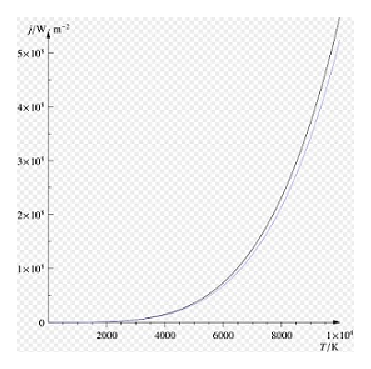
\includegraphics[scale=0.80]{mm20b019/mm20b019.eps}
        \end{center}
        \caption{MM20B019}
        \label{graph}
\end{figure}

The Stefan–Boltzmann law describes the power radiated from a black body in terms of its temperature where

\begin{itemize}
        \item $j^{\star}$ is the black-body radiant emittance (radiant flux emitted by a surface per unit area).
%        \item $\sigma$ is called the Stefan–Boltzmann constant.The value of the constant is {\displaystyle \sigma ={\frac {2\pi ^{5}k^{4}}{15c^{2}h^{3}}}=5.670374\ldots \times 10^{-8}\,\mathrm {W\,m^{-2}\,K^{-4}} .}

        \item $T$ is the thermodynamic temperature (in kelvins).
        \item $P$ is the total power radiated from an object.
        \item $A$ is the surface area of the object.
        \item $\varepsilon$ is the emissivity of the grey body.

\end{itemize}

\subsection{Description}

\begin{itemize}

    \item The equation~\ref{eqn:stefboltz} is Stefan-Boltzmann's law and the equation~\ref{eqn2:stefboltz} can be derived for a general grey body.

    \item The Stefan–Boltzmann law states that the total energy radiated per unit surface area of a black body across all wavelengths per unit time $j^{\star}$ is directly proportional to the fourth power of the black body's thermodynamic temperature T.

    \item Graph~\ref{graph} of a function of total emitted energy of a black body $j^{\star}$ proportional to its thermodynamic temperature T. In blue is total energy according to the Wien approximation.

\end{itemize}

\subsection{Further Reading}

\begin{itemize}

    \item Laboratory experiments to demonstrate the Stefan–Boltzmann radiation law using the tungsten filament of a traditional incandescent lamp have been described several times.~\cite{Marcello}

    \item The Bureau International des Poidset Mesures (International Bureau of Weights and Measures) recognized that the Planck’s law is not accurate at temperatures below the silver point (infrared radiation) and recommended using the Sakuma-Hattori equations instead of the Planck’s equation. These changes should lead naturally to modifications of the integral law of thermal radiation, the Stefan-Boltzmannn law, but apparently no such empirical correction was suggested, even though the deviations are significant or even larger than the Stefan-Boltzmann radiation.~\cite{Yuri}

\end{itemize}

%\cite{Yuri}

%\bibliography{team-3.bib}
%\bibliographystyle{plain}

1 \href{https://arxiv.org/pdf/1612.03199.pdf}{arxiv.org}

2 \href{https://www.researchgate.net/publication/258757261_Stefan-Boltzmann_law_for_the_tungsten_filament_of_a_light_bulb_Revisiting_the_experiment/link/5954d3ea0f7e9b2da1b3b8ab/download}{researchgate.net}

3 \href{https://en.wikipedia.org/wiki/Stefan%E2%80%93Boltzmann_law}{wikipedia.org}

%\end{document}
                   
